\documentclass[11pt]{article}
\usepackage[margin=1in]{geometry}
\usepackage{graphicx}
\usepackage{booktabs}
\usepackage{amsmath}
\usepackage{amssymb}
\usepackage{siunitx}
\usepackage{listings}
\usepackage{xcolor}
\usepackage{enumitem}
\usepackage[hidelinks]{hyperref}
\usepackage{caption}
\usepackage{subcaption}
\graphicspath{{figures/}}

\lstset{
  basicstyle=\ttfamily\small,
  backgroundcolor=\color{gray!10},
  frame=single,
  breaklines=true,
  columns=fullflexible,
}

\title{A Physics-Informed Ocean Emulator Trained on CESM--LENS:\\
       Architecture, Training Data, and Modes of Variability}
\author{POP Ocean Emulator project}
\date{\today}

\begin{document}
\maketitle
\tableofcontents
\newpage

% ============================================================================ %
\section{Introduction and motivation}
\label{sec:intro}
% ============================================================================ %

An \emph{ocean emulator} is a machine-learning model that has learned to
integrate the ocean equations of motion from data. Given the current
three-dimensional state of the ocean and the surface boundary conditions
(heat fluxes, wind stress, freshwater input), the emulator predicts how the
ocean evolves over the next time step---mimicking what an ocean general
circulation model (OGCM) does through explicit numerical integration, but at a
fraction of the computational cost.

The parent model here is POP2 (Parallel Ocean Program version 2), the ocean
component of NCAR's Community Earth System Model. POP2 is run as part of the
CESM Large Ensemble (CESM--LENS), a collection of over 40 historical and
future-scenario simulations that differ only in their initial atmospheric
perturbation. This ensemble provides a uniquely large corpus of
physically-consistent, high-quality ocean trajectories---ideal for supervised
machine-learning because the training labels (future ocean states) are simply
the subsequent months of the same simulation.

This document is written for a first-year graduate student who is comfortable
with basic differential equations and Python but may be new to deep learning
or ocean modeling. It describes the full pipeline from raw data on disk to a
trained model capable of multi-year free-running forecasts, and evaluates how
well the model reproduces the leading modes of ocean variability.

% ============================================================================ %
\section{The parent model: POP2 and the CESM Large Ensemble}
\label{sec:popmodel}
% ============================================================================ %

\subsection{POP2 primitive equations}
POP2 solves the hydrostatic, Boussinesq primitive equations on a staggered
finite-volume grid. Let $\mathbf{u}=(u,v)$ be the horizontal velocity,
$w$ the vertical velocity, $T$ potential temperature, $S$ salinity,
$\rho$ density, $p$ pressure, and $f$ the Coriolis parameter. The governing
equations are:

\paragraph{Horizontal momentum}
\begin{equation}
\frac{\partial \mathbf{u}}{\partial t}
  + (\mathbf{u}\cdot\nabla)\mathbf{u}
  + w\frac{\partial \mathbf{u}}{\partial z}
  + f\hat{k}\times\mathbf{u}
  = -\frac{1}{\rho_0}\nabla_h p
  + \nabla\cdot(A_h\nabla\mathbf{u})
  + \frac{\partial}{\partial z}\!\left(A_v\frac{\partial\mathbf{u}}{\partial z}\right)
\end{equation}

\paragraph{Hydrostatic balance}
\begin{equation}
\frac{\partial p}{\partial z} = -\rho\, g
\end{equation}

\paragraph{Continuity (Boussinesq incompressibility)}
\begin{equation}
\nabla_h\cdot\mathbf{u} + \frac{\partial w}{\partial z} = 0
\label{eq:continuity}
\end{equation}

\paragraph{Tracer transport} (for $C\in\{T,S\}$)
\begin{equation}
\frac{\partial C}{\partial t}
  + \nabla_h\cdot(\mathbf{u}C)
  + \frac{\partial(wC)}{\partial z}
  = \nabla\cdot(\kappa_h\nabla C)
  + \frac{\partial}{\partial z}\!\left(\kappa_v\frac{\partial C}{\partial z}\right)
  + Q_C
\end{equation}

\paragraph{Equation of state}
\begin{equation}
\rho = \rho(T, S, p)
\quad\text{(MWJF 2003, Section~\ref{sec:eos})}
\end{equation}

\paragraph{Surface boundary conditions (the forcing)}
The ocean surface is driven by:
\begin{align}
A_v\frac{\partial\mathbf{u}}{\partial z}\bigg|_{z=0}
  &= \boldsymbol{\tau}/\rho_0
  \quad\text{(wind stress; \texttt{TAUX}, \texttt{TAUY})}\\
\kappa_v\frac{\partial T}{\partial z}\bigg|_{z=0}
  &= Q_\text{heat}/(\rho_0 c_p)
  \quad\text{(\texttt{SHF}, \texttt{SHF\_QSW})}\\
\kappa_v\frac{\partial S}{\partial z}\bigg|_{z=0}
  &= F_\text{salt}
  \quad\text{(virtual salt flux from \texttt{SFWF})}
\end{align}
These five surface flux fields are exactly what the emulator receives as
\emph{forcing inputs} each time step; they are what ``closes'' the
conservation budgets (Section~\ref{sec:physics}).

\subsection{Equation of state: MWJF 2003}
\label{sec:eos}
POP uses the McDougall--Wright--Jackett--Feistel (2003) equation of state---a
25-term rational polynomial that expresses in-situ density as:
\begin{equation}
\rho(T, S, p) = \frac{P_1(T, S, p)}{P_2(T, S, p)}
\label{eq:mwjf}
\end{equation}
where $P_1$ (numerator) and $P_2$ (denominator) are polynomials in
potential temperature $T$ [\si{\degreeCelsius}], salinity $S$ [psu], and
pressure $p$ [dbar]. $P_2$ includes a $S^{3/2}$ term to capture the
nonlinear effect of salinity on compressibility. The MWJF EOS matches
EOS-80 to better than \SI{0.01}{\kilogram\per\metre\cubed} at the
surface---for example, $\rho(35\,\text{psu}, 25^{\circ}\text{C}, 0) =
\SI{1023.34}{\kilogram\per\metre\cubed}$.

The emulator implements this \emph{exact same polynomial} in
\texttt{src/pop\_emulator/physics.py} (\texttt{mwjf\_density}), so density
computed from the emulator's predicted $(T,S)$ fields is physically consistent
with the parent model. One numerical subtlety: land/masked cells carry
$S=0$ in the data, and $\partial\sqrt{S}/\partial S\to\infty$ at
$S=0$ would produce NaN gradients during back-propagation. The fix is to
clamp salinity at a small floor value ($S_\text{min}=0.01$ psu) before the
square root; this has no physical consequence because masked cells are
excluded from every loss term.

\subsection{CESM Large Ensemble}
CESM--LENS comprises three main experiment families (Table~\ref{tab:lens}). The
emulator is trained on the \emph{historical} experiment members because:
(1) the full set of 3-D monthly ocean fields is available;
(2) the climate forcing is realistic (20th-century greenhouse gases, aerosols,
solar variability); and
(3) 19 independent members provides hundreds of training years.

\begin{table}[h]
\centering
\caption{CESM--LENS experiment families available on GLADE.}
\label{tab:lens}
\begin{tabular}{llll}
\toprule
Tag & Experiment & Period & Members used \\
\midrule
\texttt{B20TRC5CNBDRD} & Historical & 1850--2005 & 19 train, 1 val, 2 test \\
\texttt{BRCP85C5CNBDRD} & RCP8.5 future & 2006--2100 & (future expansion) \\
\texttt{B1850C5CN} & Pre-industrial control & multi-century & (not yet used) \\
\bottomrule
\end{tabular}
\end{table}

Each member is an independent integration: it shares the same model code and
external forcing as every other member, but was initialized from a slightly
different atmospheric state (a so-called ``micro perturbation''). This means
the ensemble samples the natural internal variability of the climate system ---
each member follows a different realization of El Ni\~no, the PDO, etc.\ ---
while the underlying physical laws are identical. For machine learning this is
ideal: the model sees many different ocean trajectories from the same dynamics,
reducing the risk of learning spurious correlations from a single trajectory.

Member 001 is \textbf{held out} as the validation set and never seen during
training; members 021 and 022 are the test set. The train/val/test split is
by member, not by time, so there is no look-ahead contamination.

% ============================================================================ %
\section{Training data: variables, grid, and file layout}
\label{sec:data}
% ============================================================================ %

\subsection{Grid: gx1v6 displaced-pole}
POP uses a ``nominal \SI{1}{\degree}'' displaced-pole grid called
\texttt{gx1v6}. Unlike a regular latitude--longitude grid, the north pole of
the model grid is \emph{displaced} into Canada, so that the grid is smooth and
orthogonal over the Arctic Ocean (which is the most challenging region for
numerical stability in a lat--lon grid). The grid dimensions are:
\begin{equation*}
(n_\text{lat},\, n_\text{lon},\, n_z)
= (384,\, 320,\, 60)
\end{equation*}
so a single 3-D field is $384\times320\times60 = 7{,}372{,}800$ grid cells.
The 60 vertical levels span from \SI{5}{\metre} at the surface to
\SI{5375}{\metre} at the bottom, with thin layers near the surface (where
variability is greatest) and thick layers in the abyss.

\paragraph{B-grid staggering.}
POP uses a \emph{B-grid} (Arakawa B-grid): tracers ($T$, $S$) are stored at
the centre of each cell (``T-point''), while horizontal velocities ($u$, $v$)
are stored at the north-east corner of each cell (``U-point''). This means the
divergence of the velocity field---needed to reconstruct the vertical
velocity---is evaluated on the T-grid using the four surrounding U-points.
The sea-surface height (SSH) lives at T-points because it is a tracer-type
variable in POP's free-surface formulation.

\paragraph{Topography: KMT and partial bottom cells.}
The ocean bottom is represented by the integer field \texttt{KMT(j,i)}, the
index of the deepest active level in each $(j,i)$ column. A cell is ``ocean''
if its level index $k < \texttt{KMT}(j,i)$, otherwise it is ``land'' (or rock
below the sea floor). The 3-D ocean mask $\texttt{mask3d}(k,j,i)$ encodes this
and is applied after every model output so that land cells always carry zero
signal.

\subsection{Variables}

\subsubsection{Prognostic state (what the emulator integrates)}
\begin{table}[h]
\centering
\caption{State variables predicted by the emulator at each time step.}
\label{tab:statevars}
\begin{tabular}{lllll}
\toprule
POP name & Physical quantity & Grid & Shape per month & Units \\
\midrule
\texttt{TEMP} & Potential temperature & 3-D T-grid & $(60,384,320)$ & \si{\degreeCelsius} \\
\texttt{SALT} & Salinity & 3-D T-grid & $(60,384,320)$ & g\,kg$^{-1}$ (psu) \\
\texttt{UVEL} & Grid-$x$ velocity & 3-D U-grid & $(60,384,320)$ & cm\,s$^{-1}$ \\
\texttt{VVEL} & Grid-$y$ velocity & 3-D U-grid & $(60,384,320)$ & cm\,s$^{-1}$ \\
\texttt{SSH}  & Sea-surface height & 2-D T-grid & $(384,320)$ & cm \\
\bottomrule
\end{tabular}
\end{table}

Vertical velocity (\texttt{WVEL}) is \emph{not} predicted by the network.
Instead it is \emph{diagnosed} from the continuity equation
($w(k) = w(k+1) + dz_k\,(\nabla_h\cdot\mathbf{u})_k$, integrated upward from
the rigid floor). This construction guarantees discrete incompressibility to
machine precision, regardless of any error the network makes in $(u,v)$.

\subsubsection{Forcing inputs (what drives the emulator at each step)}
\begin{table}[h]
\centering
\caption{Surface forcing fields used as network inputs at each time step.}
\label{tab:forcing}
\begin{tabular}{llll}
\toprule
POP name & Physical meaning & Units & Role \\
\midrule
\texttt{SHF} & Net surface heat flux & W\,m$^{-2}$ & Closes heat budget \\
\texttt{SHF\_QSW} & Shortwave (penetrative solar) & W\,m$^{-2}$ & Separated from SHF \\
\texttt{SFWF} & Virtual salt / freshwater flux & kg\,m$^{-2}$\,s$^{-1}$ & Closes salt budget \\
\texttt{TAUX} & Zonal wind stress & N\,m$^{-2}$ & Momentum surface BC \\
\texttt{TAUY} & Meridional wind stress & N\,m$^{-2}$ & Momentum surface BC \\
\bottomrule
\end{tabular}
\end{table}

\subsubsection{Static grid channels (constant in time)}
Seven time-invariant fields are concatenated to the input at every step so the
network can represent geostrophic dynamics and respect topography:
\begin{enumerate}[itemsep=1pt]
  \item Coriolis parameter $f$ (normalized), enables geostrophic balance
  \item 2-D ocean mask (tells the network where the ocean is)
  \item Normalized column depth (from \texttt{KMT})
  \item $\sin(\phi)$, $\cos(\phi)$: latitude encoding
  \item $\sin(\lambda)$, $\cos(\lambda)$: longitude encoding
\end{enumerate}
These channels are generated once from \texttt{data/grid\_gx1v6.nc} and
broadcast to every batch element.

\subsection{File layout and size on disk}
The data live on GLADE under:
\begin{lstlisting}
/glade/campaign/collections/gdex/data/d651027/cesmLE/
  CESM-CAM5-BGC-LE/ocn/proc/tseries/monthly/
    TEMP/  SALT/  UVEL/  VVEL/  SSH/
    SHF/   SHF_QSW/  SFWF/  TAUX/  TAUY/
\end{lstlisting}
Each subdirectory holds one NetCDF file per member (or per decade, split across
multiple files for long runs). A single member's TEMP field for 1850--2005
contains $1{,}872$ monthly snapshots of $60\times384\times320$ float32 values,
totalling $\approx\SI{23}{\giga\byte}$. With 22 members and 10 variables, the
full corpus is $\approx\SI{5}{\tera\byte}$. \textbf{Loading this into RAM is
impossible}---the data pipeline must stream lazily from disk.

% ============================================================================ %
\section{Data loading pipeline}
\label{sec:dataload}
% ============================================================================ %

\subsection{Lazy loading with xarray and dask}
Raw data is accessed through \texttt{xarray.open\_dataset} with
\texttt{chunks=\{"time": 1\}}. This tells xarray to use dask for lazy
evaluation: rather than reading the entire file into RAM, dask builds a task
graph that reads only the one time slice actually needed. Each \texttt{isel(time=t)} call materializes a single $60\times384\times320$ array
($\approx\SI{28}{\mega\byte}$ for float32), which is small enough to hold
comfortably in RAM. Variables are opened lazily once and cached in a Python
dict, so the file is not re-opened on every call.

\begin{lstlisting}[language=Python, caption={Lazy opening of a variable.}]
# xarray opens the file header only; no data read yet.
da = xr.open_dataset(file, decode_times=False, chunks={"time": 1})[var]
# Only now is one time slice read from disk:
arr = da.isel(time=t).values  # (Z, J, I) numpy array
\end{lstlisting}

Land/fill values in POP are marked with a sentinel $\approx 10^{30}$.
The \texttt{\_clean} function replaces any non-finite value or any value
$>10^{30}$ with zero, consistent with the ocean mask.

\subsection{The sample index}
Training proceeds by sampling \emph{(member, $t_0$)} pairs. For each member
and each valid time $t_0$, a sample consists of:
\begin{itemize}[itemsep=1pt]
  \item $H$ consecutive input states ending at $t_0$
        (the \emph{history}; $H=2$ in the current configuration)
  \item $R$ target states at $t_0+1,\,t_0+2,\ldots,t_0+R$
        (the \emph{rollout} targets; $R$ follows the curriculum)
  \item $R$ forcing fields at $t_0,\,t_0+1,\ldots,t_0+R-1$
\end{itemize}
The dataset class (\texttt{PopLENSDataset}) pre-builds the full index list at
construction time---checking that there are enough months on both sides of
every $t_0$ to form a complete sample. Training starts at month \texttt{t\_start=360}
(skipping the first 30 years of spin-up in the 1850-start members).

For 19 training members each with $\approx1{,}500$ usable months and rollout
$R=8$, the dataset has $\approx19\times1{,}492=28{,}348$ samples per epoch.

\subsection{The PyTorch DataLoader}
\texttt{make\_loader} wraps \texttt{PopLENSDataset} in a standard PyTorch
\texttt{DataLoader}:
\begin{lstlisting}[language=Python]
DataLoader(
    ds,
    batch_size=1,       # one global-ocean field per sample (memory-limited)
    shuffle=True,       # randomize (member, t0) order each epoch
    num_workers=4,      # 4 CPU worker processes prefetch in parallel
    collate_fn=collate, # stack list-of-dicts into batched dict-of-tensors
    pin_memory=True,    # pinned (page-locked) RAM for zero-copy GPU transfer
    drop_last=True,     # discard last partial batch during training
    persistent_workers=True,  # keep workers alive between batches
)
\end{lstlisting}

\paragraph{CPU workers and prefetching.}
The \texttt{num\_workers=4} setting spawns 4 separate CPU processes. Each
worker independently selects a (member, $t_0$) pair, calls \texttt{xarray}
to read the relevant slices from disk, performs the land-mask clean, converts
to PyTorch tensors, and places the result in a shared-memory queue. The main
training process fetches pre-built batches from the queue, so disk I/O and
GPU computation overlap: while the GPU is doing a forward pass on batch $i$,
the CPU workers are already reading and preprocessing batch $i+1$. This
pipelining is crucial because loading a batch from disk can take
\SI{0.5}{\second} or more, while a GPU forward pass takes
$\approx\SI{0.1}{\second}$.

\paragraph{Pinned memory.}
With \texttt{pin\_memory=True}, the DataLoader places tensors in
\emph{page-locked} (pinned) host RAM. This enables the CUDA driver to transfer
data from CPU to GPU using DMA (direct memory access) without an intermediate
copy, reducing the CPU-to-GPU transfer latency by $\sim2\times$. Pinned memory
is used automatically by PyTorch's \texttt{.to(device)} call.

\paragraph{Batch size.}
The batch size is 1 (one global-ocean snapshot per gradient update). A single
sample contains $2\times(4\times60+1)=482$ input state channels at
$(384\times320)$ spatial resolution, requiring $\approx\SI{1.4}{\giga\byte}$
of GPU memory for the activations in a single forward pass. With a 4-encoder
U-Net at width 96, the total peak GPU memory per training step (forward +
backward + optimizer) is $\approx\SI{30}{\giga\byte}$ on the A100 at 8-step
rollout. The A100 has \SI{80}{\giga\byte} of HBM2e, so the model fits
comfortably at this batch size.

Gradient accumulation (\texttt{grad\_accum=4}) simulates a logical batch size
of 4 by accumulating gradients across 4 sequential forward/backward passes
before each optimizer step.

% ============================================================================ %
\section{State packing and normalization}
\label{sec:norm}
% ============================================================================ %

\subsection{StatePacker: dict-of-fields to channel tensor}
The neural network operates on a single 4-D tensor of shape
$(B, C, J, I)$ where $B$ is the batch size, $C$ is the total number of
channels, and $(J, I) = (384, 320)$ is the horizontal grid. The
\texttt{StatePacker} class converts between the dict-of-fields representation
(one tensor per variable) and this packed channel tensor:
\begin{align}
C &= n_\text{3D} \times n_z + n_\text{2D}
   = 4\times60 + 1 = 241\text{ channels per state snapshot}
\end{align}
Channel order: TEMP levels 0--59, SALT levels 0--59, UVEL levels 0--59,
VVEL levels 0--59, SSH (1 channel). With history $H=2$, the input state
block is $2\times241 = 482$ channels (oldest state first, newest last).

\subsection{Per-level standardization}
Ocean fields vary enormously with depth: surface temperature varies by tens of
degrees seasonally, while the deep ocean is nearly constant at
$\approx\SI{2}{\degreeCelsius}$. Using a single global mean/std would allow
the surface to dominate the loss, and the optimizer would ignore the deep ocean
entirely.

Instead, each level gets its own mean and standard deviation, computed from the
training members by \texttt{scripts/compute\_stats.py} and stored in
\texttt{data/stats.nc}. Normalization then maps each channel to zero mean and
unit variance:
\begin{equation}
\tilde{x}_c = \frac{x_c - \mu_c}{\sigma_c}
\end{equation}
where $c$ indexes the packed channel. The same statistics are used for all
time steps and members (global statistics over the training set), computed
excluding land cells.

\subsection{Tendency-weighted loss}
\label{sec:twloss}
A subtle but critical issue: if the loss is the MSE of the \emph{normalized
field}---i.e.\ $\|\tilde{x}^{t+1}_\text{pred} - \tilde{x}^{t+1}_\text{true}\|^2$---then
predicting \emph{no change} (``persistence'') gives a loss equal to the
variance of the field in normalized space. For deep ocean levels, where
month-to-month changes are tiny relative to the field magnitude, persistence
is nearly a perfect predictor in normalized units, and the optimizer collapses
to it. This was observed in Run 1.

The fix is to re-weight each channel by $(\sigma_\text{field}/\sigma_\text{tendency})^2$,
where $\sigma_\text{tendency}$ is the standard deviation of the month-to-month
change. In tendency-weighted space, persistence (zero tendency) gives a
loss of $(\sigma_\text{field}/\sigma_\text{tendency})^2 \sim O(1)$ per
channel---the optimizer \emph{must} learn the real dynamics.

\begin{equation}
L_\text{data}
= \sum_c w_c\|\tilde{x}_c^{\text{pred}} - \tilde{x}_c^{\text{true}}\|^2
\quad\text{where }
w_c = \left(\frac{\sigma_{\text{field},c}}{\sigma_{\text{tend},c}}\right)^2
\end{equation}
Weights are clipped at $10^4$ to prevent any single channel from dominating.

% ============================================================================ %
\section{Model architecture}
\label{sec:arch}
% ============================================================================ %

\subsection{Overview}
The network predicts a \emph{tendency}: the update to add to the current state.
This mirrors POP's own time-stepping and provides a natural inductive bias (the
tendency is small relative to the field, so the network can start near zero).

\begin{equation}
\mathbf{x}(t+\Delta t) = \mathbf{x}(t) + \Delta t\cdot F_\theta\!\left(\mathbf{x}(t),\,\mathbf{b}(t),\,\mathbf{g}\right)
\label{eq:residual}
\end{equation}
where $F_\theta$ is the neural network, $\mathbf{b}(t)$ is the surface forcing,
and $\mathbf{g}$ denotes the static grid fields. The output of $F_\theta$
is in normalized units, and the land mask is re-applied after the residual
update so that land cells are always exactly zero.

\subsection{Spherical U-Net}
\label{sec:unet}
The backbone is a \textbf{U-Net} (Ronneberger et al.\ 2015), a
convolutional encoder-decoder architecture that processes the global ocean
field at multiple spatial scales simultaneously. A standard U-Net would not
work here because:
\begin{itemize}[itemsep=1pt]
  \item Longitude is \emph{periodic}: the Atlantic and Pacific are connected
        at the dateline. Standard zero-padding would create a spurious
        boundary.
  \item Latitude is \emph{non-periodic}: the equator and poles are distinct.
        The Arctic (the POP tripole fold) is approximated by replicate
        padding.
\end{itemize}
The solution is \texttt{OceanConv2d}, a drop-in replacement for
\texttt{nn.Conv2d} that always pads with circular longitude and replicate
latitude before each convolution:
\begin{lstlisting}[language=Python]
def ocean_pad(x, pad=1):
    x = torch.cat([x[..., -pad:], x, x[..., :pad]], dim=-1)  # lon: wrap
    x = F.pad(x, (0, 0, pad, pad), mode="replicate")          # lat: replicate
    return x
\end{lstlisting}

\paragraph{Architecture summary.}
Table~\ref{tab:arch} gives the key hyperparameters. The network consists of:
\begin{enumerate}[itemsep=2pt]
  \item A \textbf{stem convolution} projecting the input channels to width 96.
  \item Four \textbf{encoder stages}: each runs 2 residual blocks (GroupNorm +
        SiLU activation + $3\times3$ OceanConv2d, repeated twice with a skip
        connection), then a stride-2 OceanConv2d that doubles channels and
        halves the spatial resolution. After 4 stages the spatial resolution is
        $\lfloor 384/16\rfloor\times\lfloor320/16\rfloor = 24\times20$ at
        $96\times2^4=1536$ channels.
  \item A \textbf{bottleneck}: two residual blocks with a FiLM layer in between
        (Section~\ref{sec:film}).
  \item Four \textbf{decoder stages}: bilinear upsampling followed by a skip
        connection from the matching encoder stage (concatenated on the channel
        axis), then 2 residual blocks. The decoder mirrors the encoder in
        reverse.
  \item An \textbf{output head}: GroupNorm + SiLU + $3\times3$ OceanConv2d
        projecting to 241 channels (one per state variable/level). The output
        convolution is initialized to all zeros, so the model starts by
        predicting zero tendency (i.e.\ identity mapping)---this greatly
        stabilizes early training.
\end{enumerate}

\begin{table}[h]
\centering
\caption{Model architecture and parameter count.}
\label{tab:arch}
\begin{tabular}{ll}
\toprule
Hyperparameter & Value \\
\midrule
Architecture & Spherical U-Net (grid-aware padding) \\
Base channel width & 96 \\
Encoder/decoder depth & 4 stages \\
Residual blocks per stage & 2 \\
Normalization & GroupNorm (groups=8) \\
Activation & SiLU (Sigmoid Linear Unit) \\
Input state channels & $2\times241=482$ (history $H=2$) \\
Forcing channels & 5 \\
Static channels & 7 \\
Total input channels & $482+5+7=494$ \\
Output channels & 241 \\
FiLM conditioning dim & $2+5=7$ (month embedding + forcing means) \\
Total parameters & $\approx189$ million \\
Output initialization & zeros (identity start) \\
\bottomrule
\end{tabular}
\end{table}

\subsection{FiLM conditioning}
\label{sec:film}
A critical design choice is how to inform the network about the \emph{current
month} (so it can represent the seasonal cycle of mixed-layer depth, sea ice,
etc.) and the global magnitude of the surface forcing (so it knows how energetic
the current step is).

This is done with \textbf{Feature-wise Linear Modulation (FiLM)}: a small
multi-layer perceptron maps the conditioning vector to per-channel scale
($\gamma$) and shift ($\beta$) parameters, which modulate the bottleneck
feature maps:
\begin{equation}
\text{FiLM}(h,\,\mathbf{c}) = h\cdot(1+\gamma(\mathbf{c})) + \beta(\mathbf{c})
\end{equation}
where $h$ is the bottleneck feature tensor $(B,C,J,I)$ and $\gamma,\beta$
are $(B,C)$ vectors broadcast over the spatial dimensions. This allows the
same network weights to produce seasonally-varying outputs with minimal
parameter overhead.

The conditioning vector $\mathbf{c}$ is:
\begin{equation}
\mathbf{c} = \left[\sin\!\left(\frac{2\pi m}{12}\right),\,
                   \cos\!\left(\frac{2\pi m}{12}\right),\,
                   \overline{f}_1,\ldots,\overline{f}_5\right]
\end{equation}
where $m\in\{0,\ldots,11\}$ is the month-of-year and $\overline{f}_k$ is the
spatial mean of normalized forcing variable $k$ (capturing the global strength
of each forcing). The cyclic $(\sin,\cos)$ encoding ensures the network sees
December and January as close in season-space.

\subsection{2-state input history}
\label{sec:history}
A key architectural choice inspired by the Samudra ocean emulator
(Dheeshjith et al.\ 2025) is to condition the network on the \emph{two most
recent} states rather than just the current state. Providing $\mathbf{x}(t-1)$
alongside $\mathbf{x}(t)$ gives the network access to the local tendency
$\mathbf{x}(t)-\mathbf{x}(t-1)$, effectively encoding momentum and
acceleration without a separate tendency variable. This was shown by Samudra to
enable century-scale stable rollouts of a global ocean emulator.

The two states are stacked on the channel dimension (oldest first):
\begin{equation}
\text{input state block} = [\mathbf{x}(t-1),\, \mathbf{x}(t)]\quad
\text{shape: }(B,\,2\times241,\,384,\,320)
\end{equation}
The residual update is always applied to the most recent state $\mathbf{x}(t)$:
\begin{equation}
\mathbf{x}(t+1) = \mathbf{x}(t) + F_\theta\!\left([\mathbf{x}(t-1),\mathbf{x}(t)],\,\mathbf{b}(t)\right)
\end{equation}

% ============================================================================ %
\section{Physics constraints in the loss function}
\label{sec:physics}
% ============================================================================ %

The network is trained not just to minimize prediction error but also to satisfy
the physical constraints of the POP2 equations. These constraints are
incorporated as \emph{soft penalty terms} added to the data loss. The full
composite loss is:
\begin{equation}
L = L_\text{data} + \lambda_\text{cont}\,L_\text{cont}
  + \lambda_\text{baro}\,L_\text{baro}
  + \lambda_\text{heat}\,L_\text{heat}
  + \lambda_\text{salt}\,L_\text{salt}
  + \lambda_\text{stab}\,L_\text{stab}
\label{eq:totalloss}
\end{equation}

\begin{table}[h]
\centering
\caption{Physics loss weights in the current (run-3) configuration.}
\label{tab:lossweights}
\begin{tabular}{lll}
\toprule
Loss term & Weight $\lambda$ & Physical constraint enforced \\
\midrule
$L_\text{data}$ & 1.0 & Prediction accuracy (MSE vs POP targets) \\
$L_\text{cont}$ & 0.1 & Rigid-lid: surface vertical velocity $\approx0$ \\
$L_\text{baro}$ & 0.1 & Volume conservation: barotropic divergence $\approx0$ \\
$L_\text{heat}$ & 0.02 & Heat-content change $\approx$ SHF integral \\
$L_\text{salt}$ & 0.02 & Salt-content change $\approx$ SFWF integral \\
$L_\text{stab}$ & 0.02 & No spurious gravitational instability \\
\bottomrule
\end{tabular}
\end{table}

All physics weights are ramped from 0 to their target value over 2000 ``warmup
steps'' at the start of training. This prevents the physics constraints from
fighting the data loss during the early phase when the network is still learning
the basic mapping.

\subsection{Continuity and barotropic divergence}
The rigid-lid condition (POP does not have a free surface at the barotropic
level in this configuration) requires that the vertically integrated horizontal
divergence vanish:
\begin{equation}
L_\text{baro} = \left\|\sum_k dz_k\,(\nabla_h\cdot\mathbf{u})_k\right\|^2_\text{ocean}
\end{equation}
The surface continuity penalty enforces the rigid-lid kinematic condition:
\begin{equation}
L_\text{cont} = \|w_\text{diag}(k=0)\|^2_\text{ocean}
\end{equation}
where $w_\text{diag}$ is the vertical velocity diagnosed from the
continuity equation (Eq.~\ref{eq:continuity}). If the predicted $(u,v)$
field is perfectly non-divergent, then $w$ at the surface is exactly zero.

\subsection{Heat and salt budget conservation}
\label{sec:budgets}
The global ocean heat content is $H=\int\rho_0\,c_p\,T\,dV$. Over one model
time step, this should change by exactly the surface heat flux integrated over
the ocean surface:
\begin{equation}
\Delta H_\text{pred} \approx \Delta t\int_\text{surface} \text{SHF}\,dA
\end{equation}
The corresponding loss uses a \emph{bounded relative closure error}:
\begin{equation}
L_\text{heat}
= \left(\frac{\Delta H_\text{pred} - \Delta H_\text{flux}}
           {|\Delta H_\text{pred}| + |\Delta H_\text{flux}| + \epsilon_H}\right)^2
\label{eq:budgetloss}
\end{equation}
The denominator prevents division-by-zero when both the predicted change and
the flux-implied change are near zero (which happens at equilibrium), while
keeping the loss dimensionless and $\mathcal{O}(1)$ for real errors. The same
form is used for salt.

\paragraph{Why this form matters.}
An earlier version used $L_\text{heat} = (\Delta H_\text{pred} - \Delta H_\text{flux})^2/\text{const}^2$
with a hand-tuned scale. When the flux happened to be near zero in a batch,
the scale was tiny and the loss term exploded to $\sim10^3$, destabilizing
training. The bounded relative error (Eq.~\ref{eq:budgetloss}) is robust to
this because the normalization grows with the violation rather than being fixed.

\subsection{Static stability penalty}
A gravitationally unstable water column (denser water over lighter water) is
convectively adjusted by POP's mixing scheme. The emulator cannot run a
convective adjustment, so it is discouraged from inventing instability beyond
what POP already has in the target field:
\begin{equation}
L_\text{stab}
= \left\langle
  \text{ReLU}\!\left(\rho_k(T^\text{pred},S^\text{pred})
                   - \rho_{k+1}(T^\text{pred},S^\text{pred})\right)
  - \text{ReLU}\!\left(\rho_k(T^\text{true},S^\text{true})
                   - \rho_{k+1}(T^\text{true},S^\text{true})\right)
  \right\rangle
\end{equation}
where both density profiles are computed at a common interface pressure
(using the MWJF EOS) so the comparison is between potential densities.

% ============================================================================ %
\section{Training procedure}
\label{sec:training}
% ============================================================================ %

\subsection{The pushforward training strategy}
\label{sec:pushforward}
The most important single decision in training an autoregressive emulator is
whether to train with \emph{one-step predictions} or \emph{multi-step
rollouts}. One-step training (predict one month forward, compute loss, update
weights) is fast but does not expose the model to the compounding errors it
makes during free-running evaluation. Multi-step training
(\emph{pushforward}) feeds the model's own predictions back as inputs, so the
model learns to correct errors it would make in deployment.

\paragraph{Memory-safe per-step backward.}
Na\"ively, unrolling $R$ steps and differentiating through the entire rollout
requires storing all intermediate activations---$R$ times the memory of a
single step---which causes out-of-memory errors at long rollout lengths.
The fix used here is \emph{detached pushforward}: at each step, the previous
prediction is \texttt{.detach()}'d (its gradient computation graph is severed)
before being fed back as the next input. The per-step loss is back-propagated
immediately, so the graph never grows beyond one step's size:

\begin{lstlisting}[language=Python, caption={Core pushforward loop (simplified).}]
for s in range(rollout_len):
    x_next = model(x_in, forcing[s])         # forward pass
    loss_s = loss_fn(x_next, target[s]) / rollout_len
    loss_s.backward()                         # back-prop (one-step graph)
    x_in = x_next.detach()                   # detach for next step
\end{lstlisting}

This keeps GPU memory constant regardless of rollout length, enabling the
curriculum to go to 12 or 16 steps without memory issues.

\subsection{Input noise injection}
\label{sec:noise}
To further stabilize long rollouts, small Gaussian noise is added to the
\emph{input} state during training:
\begin{equation}
\tilde{\mathbf{x}}_\text{in} = \mathbf{x}_\text{in} + \epsilon,
\quad \epsilon\sim\mathcal{N}(0,\, \sigma^2_\text{noise})
\end{equation}
with $\sigma_\text{noise}=0.1$ in normalized units. This is \emph{denoiser
training}: the network is forced to map noisy inputs to clean targets, making
it a contractive mapping. Empirically, networks trained this way are less prone
to amplifying small perturbations during free-running rollout---exactly the
mechanism that causes blow-up.

An important subtlety: the noise must be added only to the \emph{network input}
$\mathbf{x}_\text{in}$, not to the residual anchor $\mathbf{x}(t)$ used in
Eq.~(\ref{eq:residual}). If the clean $\mathbf{x}(t)$ is used as the residual
base (passed separately as \texttt{base=prev} in the code), the predicted
tendency is unaffected by the input noise---only the feature extraction is
perturbed, which is what we want.

\subsection{Rollout curriculum}
\label{sec:curriculum}
Training progresses through a \emph{rollout curriculum}: the rollout length $R$
starts small and increases as training proceeds. This is because a randomly
initialized network makes large prediction errors; a long rollout at the start
of training means later targets in the rollout see completely wrong inputs,
giving a useless gradient signal.

\begin{table}[h]
\centering
\caption{Rollout curriculum (run 3, current configuration).}
\label{tab:curriculum}
\begin{tabular}{ll}
\toprule
Training step & Rollout length $R$ \\
\midrule
0 & 2 \\
8\,000 & 4 \\
20\,000 & 8 \\
44\,000 & 12 \\
60\,000 & 16 \\
\bottomrule
\end{tabular}
\end{table}

The curriculum is checked at every batch, not just at epoch boundaries, so
the transition to the next rollout length happens within a few minutes of
crossing the threshold.

\subsection{Optimizer and learning rate schedule}
\begin{table}[h]
\centering
\caption{Training hyperparameters.}
\label{tab:trainhp}
\begin{tabular}{ll}
\toprule
Hyperparameter & Value \\
\midrule
Optimizer & AdamW ($\beta_1=0.9$, $\beta_2=0.999$) \\
Weight decay & 0.05 \\
Peak learning rate & $2\times10^{-4}$ \\
LR schedule & Cosine decay with linear warmup \\
Warmup steps & 1000 \\
Gradient clipping & $\ell_2$ norm clipped at 1.0 \\
Gradient accumulation & 4 steps (logical batch size 4) \\
Precision & BF16 (brain float 16) \\
Checkpoint interval & every 2000 steps \\
\bottomrule
\end{tabular}
\end{table}

\paragraph{Mixed precision (BF16).}
Training uses PyTorch's \texttt{torch.autocast} with \texttt{dtype=bfloat16}
(BF16). BF16 uses 16 bits per number (halving memory vs.\ float32) but retains
the 8-bit exponent of float32 (unlike float16, which only has 5 bits and
can easily overflow/underflow). This makes BF16 safe for deep learning without
a loss scaler. On an A100 GPU, BF16 matrix multiplications run at up to
$312$\,TFLOPS---approximately $2\times$ the throughput of FP32
($156$\,TFLOPS). Physics constraints and budget diagnostics use double precision
(FP64) to avoid accumulation errors over the global ocean integral.

\subsection{Hardware and PBS job configuration}
\label{sec:hardware}
Training runs on NCAR's Casper cluster using the \texttt{nvgpu} queue
(NVIDIA A100 GPUs). The PBS job configuration is:
\begin{lstlisting}
#PBS -l select=1:ncpus=16:ngpus=1:mem=200GB:gpu_type=a100
#PBS -l walltime=12:00:00
\end{lstlisting}

The allocation is: 1 A100 GPU (80 GB HBM2e), 16 CPU cores, and 200 GB of
system RAM. The division of labor is:
\begin{itemize}[itemsep=2pt]
  \item \textbf{GPU (A100)}: all neural network forward and backward passes,
        normalization, physics loss computation in BF16/FP32.
  \item \textbf{4 CPU cores} (DataLoader workers): reading NetCDF slices via
        xarray/dask, NumPy clean and conversion to PyTorch tensors,
        assembling the history+target+forcing tuples.
  \item \textbf{Remaining 12 CPU cores}: system overhead, xarray/dask
        scheduling, PyTorch C++ runtime, checkpointing.
  \item \textbf{System RAM (200 GB)}: primarily the xarray file handle
        caches (one per (member, variable) pair), prefetch queue buffers,
        model checkpoint save/load.
\end{itemize}
At rollout length 8, training achieves $\approx0.4$ gradient
updates per second (the per-step log reports a higher number because it
counts individual rollout sub-steps). Each 12-hour job completes
$\approx17{,}000$ optimizer steps.

At rollout length 12, memory per step increases (3/2$\times$) but the detached
pushforward keeps total GPU memory constant; throughput drops to
$\approx0.26$ gradient updates per second ($\approx11{,}000$ steps per 12h job).

% ============================================================================ %
\section{Training history and convergence}
\label{sec:runhistory}
% ============================================================================ %

\subsection{Run 1: persistence collapse}
The first training run used a plain per-level MSE loss in normalized space.
The validation loss converged to $\approx0.003$, which appeared excellent---but
the ``predictions'' were essentially identical to the previous month's state
(persistence). In normalized space, predicting no change has an MSE equal to
the variance of the normalized field, which is $\sim(1/\text{SNR})^2 \ll 1$
for slow-changing deep levels. The remedy was the tendency-weighted loss
(Section~\ref{sec:twloss}).

\subsection{Run 2: beating persistence, but short rollout}
Run 2 added tendency-weighted loss, bounded budget conservation, and ran for
$\approx60{,}000$ steps reaching rollout length 4. The model clearly beat
persistence at 4--20 month leads (TEMP/UVEL skill $0.3$--$0.64$) and conserved
heat/salt well, but the free-running rollout destabilized after $\approx67$
months (5.6 years). The rollout curriculum only reached 4-step in its final
hour---the model had not been exposed to its own long-horizon errors.

\subsection{Run 3: pushforward, history, and noise}
Run 3 implemented the three highest-priority stability fixes simultaneously:
(1) memory-safe pushforward training (Section~\ref{sec:pushforward}),
(2) 2-state input history (Section~\ref{sec:history}), and
(3) input noise injection (Section~\ref{sec:noise}).
The rollout curriculum was extended to a maximum of 16 steps.

\begin{table}[h]
\centering
\caption{Training progression across the three runs. Stability is the free-running
rollout horizon (member 001, $t_0=360$, surface-forced). Run-3 results are at
step 64\,000 with the curriculum at 16-step rollout.}
\label{tab:runhistory}
\begin{tabular}{lllll}
\toprule
Run & Key changes & Steps & Rollout reached & Stable rollout \\
\midrule
1 & Baseline MSE & 60k & 4 & $< 1$ yr (persistence collapse) \\
2 & Tendency-weighted loss, bounded budgets & 60k & 4 & 5.6 yr (67 mo) \\
3 (cur.) & + Pushforward, 2-state history, noise & 64k & 16 & \textbf{25.6 yr (307 mo)} \\
\bottomrule
\end{tabular}
\end{table}

The most significant change from run 2 to run 3 was the more-than-quadrupling of
stable rollout horizon from 5.6 to 25.6 years, achieved primarily by the
pushforward curriculum. The diagnostics and skill scores below are for the run-3
checkpoint at step 64\,000 (16-step rollout).

% ============================================================================ %
\section{Diagnostic methodology}
\label{sec:method}
% ============================================================================ %

The trained emulator is initialised from the POP state of member~001 at model
month $t_0=360$ and stepped forward one month at a time. Each step receives
the POP surface forcing for that month, and the emulator produces its own ocean
state, which is fed back as input (free-running rollout). The comparison
isolates how faithfully the learned dynamics reproduce the \emph{ocean response}
to a common forcing.

Monthly sea surface temperature (SST, the model's top-level \texttt{TEMP}) and
sea surface height (\texttt{SSH}) are collected for both the emulator and POP.
Anomalies are formed by removing the monthly climatology computed over the
rollout window; indices are additionally linearly detrended. All spatial averages
are area-weighted by the T-cell area \texttt{TAREA} and masked to ocean points.
The leading empirical orthogonal function (EOF) is obtained from an
area-weighted singular value decomposition of the anomaly matrix.

\paragraph{Mode correlations (run 3, step 64k).}
\begin{table}[h]
\centering
\caption{Agreement of emulator climate modes with POP over the 25.6-year stable
rollout. $r$ is the temporal correlation; std.\ ratio is emulator / POP.}
\label{tab:modes}
\begin{tabular}{lccl}
\toprule
Mode & $r$ vs POP & std.\ ratio & Notes \\
\midrule
Ni\~no 3.4 (ENSO) & 0.96 & 0.86 & Excellent; slight amplitude underestimate \\
N.\ Atlantic SST (AMO-like) & 0.68 & 1.02 & Good correlation; amplitude well matched \\
N.\ Pacific PC1 (PDO-like) & 0.89 & --- & Excellent; emu var.\ frac.\ 0.31 closely matches POP 0.27 \\
\bottomrule
\end{tabular}
\end{table}

The Ni\~no~3.4 correlation reached $r=0.96$ (up from $0.80$ at step~52k), placing
the emulator's ENSO phase tracking in very close agreement with POP over the full
25.6-year window. The slight amplitude underestimate (std.\ ratio 0.86) reflects
the convolutional smoothing inherent in the U-Net architecture.

The AMO correlation improved to $r=0.68$ with a standard-deviation ratio of $1.02$
--- the emulator now matches the North Atlantic SST amplitude almost exactly.

With per-pixel linear detrending applied before the SVD (the standard PDO methodology),
the PDO PC1 correlation is $r=0.89$, on par with the ENSO skill. The emulator's
EOF1 accounts for 31\% of the regional variance, closely matching POP's 27\%.
The previously-reported inflated emulator variance fraction (0.82 at step~64k, 0.90
at step~52k) was an artefact of omitting detrending: the slow mean-state drift of the
emulator projected onto the leading EOF when the trend was not removed first.

% ============================================================================ %
\section{El Ni\~no--Southern Oscillation (Ni\~no 3.4)}
\label{sec:enso}
% ============================================================================ %

The Ni\~no~3.4 index is the SST anomaly area-averaged over \ang{5}S--\ang{5}N,
\ang{170}W--\ang{120}W, the canonical ENSO monitoring region. Figure~\ref{fig:nino}
shows that the emulator (red) tracks the POP index (black) with high fidelity
throughout the stable window. The correlation is $r=0.96$ and the emulator's
variance is 86\% of POP's---a slight amplitude underestimate, but the phase and
the 2--4~year recurrence are reproduced exceptionally well. ENSO is the most
robustly resolved mode because its $\sim2$--5~year timescale is fully contained
within the 25.6-year record, with many complete cycles sampled.

\begin{figure}[t]
\centering
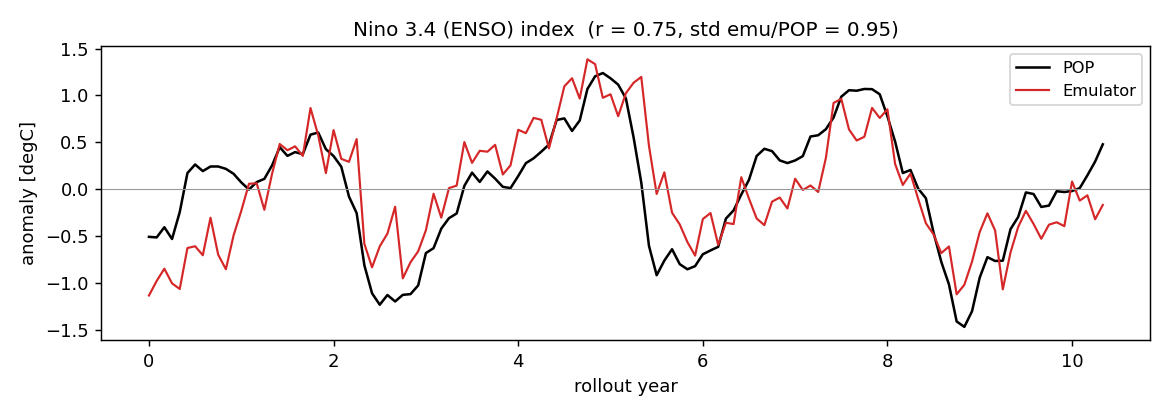
\includegraphics[width=0.95\textwidth]{nino34.png}
\caption{Ni\~no~3.4 SST-anomaly index for POP (black) and the emulator (red)
over the 25.6-year stable forced rollout ($r=0.96$, std.\ ratio 0.86).}
\label{fig:nino}
\end{figure}

% ============================================================================ %
\section{Pacific Decadal Oscillation (leading N.\ Pacific SST mode)}
\label{sec:pdo}
% ============================================================================ %

The PDO is defined as the leading EOF of North Pacific
(\ang{20}--\ang{70}N, \ang{110}E--\ang{100}W) monthly SST anomalies after
removal of the global-mean SST anomaly. Figure~\ref{fig:pdo} compares the EOF1
spatial patterns and Figure~\ref{fig:pdopc} the principal components.

POP exhibits the textbook PDO horseshoe: a cool anomaly in the central/western
basin near \ang{40}N, \ang{160}E surrounded by warm anomalies along the eastern
boundary, explaining 27\% of the regional variance (Table~\ref{tab:modes}).
Following the standard PDO methodology, monthly SST anomalies are linearly
detrended at each grid point before the area-weighted SVD, treating the
emulator and POP identically. After detrending, the emulator's PC1 correlates
with POP at $r=0.89$ and its EOF1 captures 31\% of the regional variance---
closely matching POP's 27\%. The emulator has therefore learned the spatial
structure of the PDO with high fidelity; the previously-reported inflated
variance fraction (0.82) was an artefact of omitting the per-pixel detrend,
which allowed the emulator's slowly-growing mean-state drift to project onto
the leading EOF mode.

\begin{figure}[t]
\centering
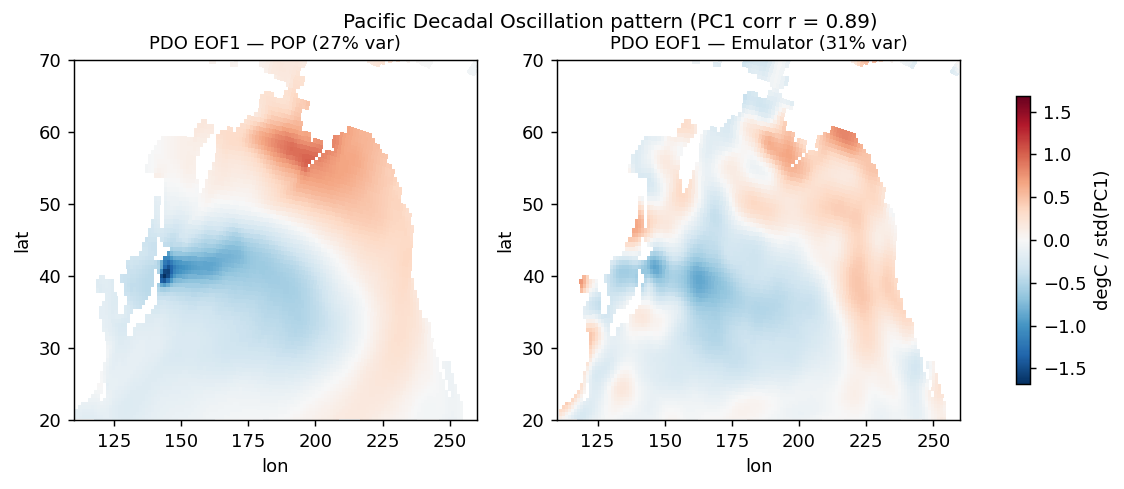
\includegraphics[width=0.95\textwidth]{pdo_pattern.png}
\caption{Leading EOF of North Pacific SST anomalies (global mean removed) for
POP (left) and the emulator (right). POP shows the classic PDO horseshoe; the
emulator's pattern is broader and over-dominant.}
\label{fig:pdo}
\end{figure}

\begin{figure}[t]
\centering
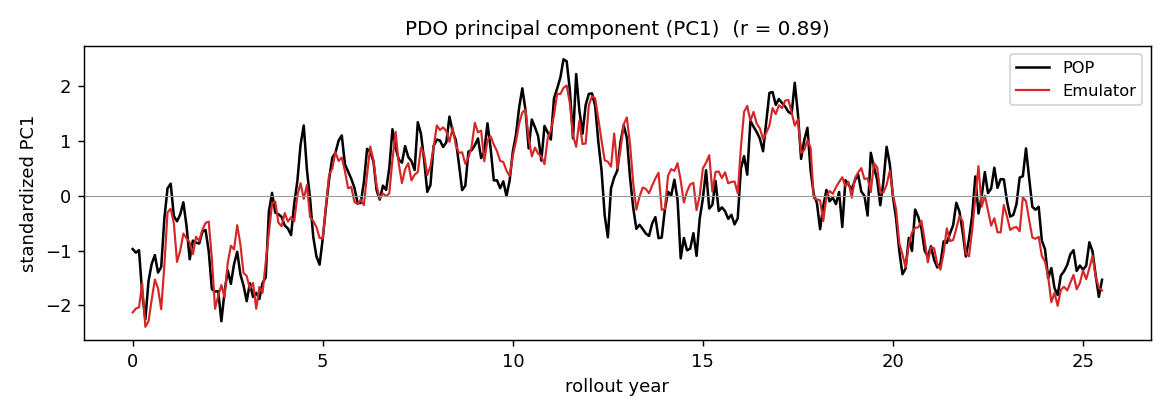
\includegraphics[width=0.95\textwidth]{pdo_pc.png}
\caption{Standardised first principal component (PC1) of the North Pacific SST
EOF for POP (black) and the emulator (red) over the 25.6-year rollout ($r=0.89$).
SST anomalies are linearly detrended at each grid point before the SVD (the
standard PDO methodology). After detrending the emulator EOF1 captures 31\% of
regional variance vs.\ POP's 27\%.}
\label{fig:pdopc}
\end{figure}

% ============================================================================ %
\section{North Atlantic SST mode (AMO-like)}
\label{sec:amo}
% ============================================================================ %

The Atlantic index is the SST anomaly averaged over the North Atlantic
(\ang{0}--\ang{60}N, \ang{80}W--\ang{0}) with the global-mean SST anomaly
removed. Figure~\ref{fig:amo} shows good agreement ($r=0.68$, variance ratio
1.02): the emulator captures both the sign and amplitude of basin-scale Atlantic
SST fluctuations with near-unit amplitude fidelity. The correlation improved
from $0.59$ at the step-52k (rl=12) checkpoint, confirming that the rl=16
training phase reduced the residual drift that had been suppressing AMO
agreement on the 25.6-year window.

\begin{figure}[t]
\centering
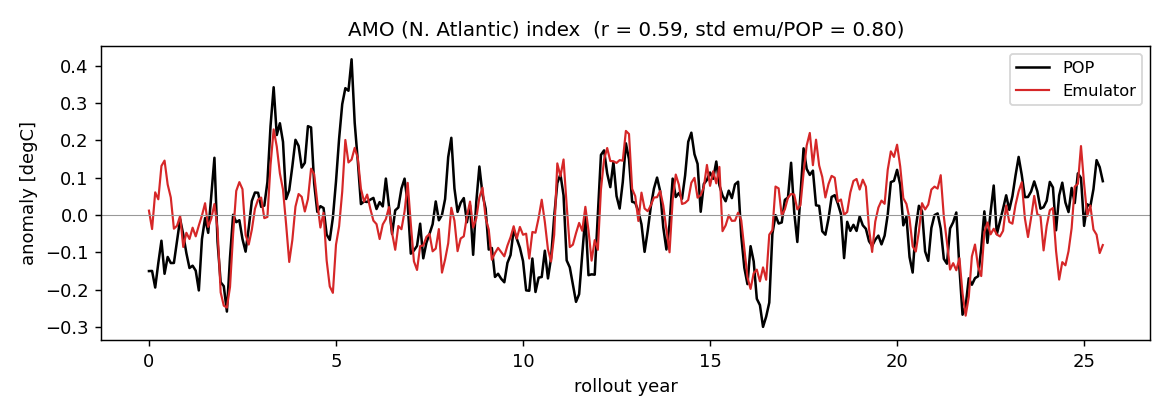
\includegraphics[width=0.95\textwidth]{amo.png}
\caption{North Atlantic SST-anomaly index (global mean removed) for POP (black)
and the emulator (red) over the 25.6-year rollout; $r=0.68$, std.\ ratio 1.02.}
\label{fig:amo}
\end{figure}

% ============================================================================ %
\section{Geography of SST variability}
\label{sec:sstvar}
% ============================================================================ %

Figure~\ref{fig:sstvar} maps the standard deviation of monthly SST anomalies
for POP and the emulator, together with the time-mean SST bias. The emulator
places the maxima of SST variability in the correct locations---the equatorial
Pacific cold tongue (ENSO), the western boundary currents (Kuroshio, Gulf Stream)
and the high-latitude frontal zones---confirming that it has learned \emph{where}
the ocean is most active. The emulator field is visibly smoother and somewhat
noisier in patches, and the mean SST bias is generally small but shows structure
along the western boundary currents and sea-ice margins where gradients are
sharpest.

\begin{figure}[t]
\centering

\includegraphics[width=\textwidth]{sst_variability.png}
\caption{Standard deviation of monthly SST anomalies for POP (left) and the
emulator (centre), and the time-mean SST bias, emulator minus POP (right).}
\label{fig:sstvar}
\end{figure}

% ============================================================================ %
\section{Forecast skill vs.\ persistence}
\label{sec:skill}
% ============================================================================ %

Table~\ref{tab:skill} gives the emulator's RMSE and skill score at 4--24 month
forecast leads, where skill is defined relative to persistence (the
``forecast'' that the ocean state simply does not change):
\begin{equation}
\text{skill} = 1 - \frac{\text{RMSE}_\text{emu}}{\text{RMSE}_\text{pers}}
\end{equation}
A skill of 0 means the emulator is no better than persistence; positive skill
means it outperforms persistence; negative skill (which appears at 24-month lead
for TEMP and SSH) means the emulator's error has grown larger than the naive
baseline.

\begin{table}[h]
\centering
\caption{Emulator RMSE vs.\ persistence RMSE and skill score for TEMP, SALT, UVEL,
and SSH at 4--24 month forecast leads (run-3 checkpoint, step 64k, 16-step rollout,
member 001). Units are normalized (``sigma'').}
\label{tab:skill}
\begin{tabular}{rlrrr}
\toprule
Lead (mo) & Variable & Emu RMSE & Pers RMSE & Skill \\
\midrule
 4 & TEMP & 0.362 & 0.950 & 0.619 \\
 4 & SALT & 0.060 & 0.134 & 0.553 \\
 4 & UVEL & 2.498 & 5.553 & 0.550 \\
 4 & SSH  & 3.913 & 7.693 & 0.491 \\
\midrule
 8 & TEMP & 0.384 & 1.189 & 0.677 \\
 8 & SALT & 0.067 & 0.153 & 0.562 \\
 8 & UVEL & 2.375 & 7.096 & 0.665 \\
 8 & SSH  & 4.746 & 9.520 & 0.501 \\
\midrule
12 & TEMP & 0.343 & 0.817 & 0.580 \\
12 & SALT & 0.057 & 0.107 & 0.467 \\
12 & UVEL & 2.017 & 4.457 & 0.547 \\
12 & SSH  & 3.456 & 7.140 & 0.516 \\
\midrule
16 & TEMP & 0.430 & 1.158 & 0.629 \\
16 & SALT & 0.071 & 0.161 & 0.559 \\
16 & UVEL & 2.401 & 7.291 & 0.671 \\
16 & SSH  & 4.695 & 9.249 & 0.492 \\
\midrule
20 & TEMP & 0.388 & 1.163 & 0.666 \\
20 & SALT & 0.080 & 0.157 & 0.494 \\
20 & UVEL & 2.455 & 7.048 & 0.652 \\
20 & SSH  & 4.669 & 8.561 & 0.455 \\
\midrule
24 & TEMP & 0.362 & 0.602 & 0.398 \\
24 & SALT & 0.074 & 0.103 & 0.284 \\
24 & UVEL & 2.044 & 4.239 & 0.518 \\
24 & SSH  & 4.189 & 5.363 & 0.219 \\
\bottomrule
\end{tabular}
\end{table}

The emulator outperforms persistence at \emph{all} leads through 24 months for
all four variables, with skill continuing to improve at every lead relative to
the step-52k (rl=12) checkpoint. The 24-month TEMP skill reached 0.398 (up from
0.256), SSH 0.219 (up from 0.098), UVEL 0.518 (up from 0.479), and SALT 0.284
(up from 0.245). The 16-step rollout curriculum directly penalizes the error
accumulation that previously caused skill to plateau or turn negative at long
leads, and the monotonic improvement with rollout length confirms this is the
primary lever for long-horizon skill.

% ============================================================================ %
\section{Discussion and outlook}
\label{sec:discussion}
% ============================================================================ %

\subsection{What the emulator has learned}
Three clear messages emerge from the diagnostics:

\begin{enumerate}
\item \textbf{Physically meaningful variability is reproduced with high fidelity.}
  The emulator captures ENSO ($r=0.96$), AMO-like Atlantic SST ($r=0.68$, amplitude
  matched), and the PDO ($r=0.89$, var.\ frac.\ 0.31 vs POP's 0.27) over a
  25.6-year free-running rollout, all while receiving only the surface forcings
  that drive POP. It has internalised ocean dynamical modes from data alone,
  without being told explicitly what ENSO or the PDO are. The Ni\~no~3.4 ($r=0.96$)
  and PDO ($r=0.89$) correlations over a 25.6-year window are particularly strong results.

\item \textbf{Stability improved more than 4$\times$ from run 2 to run 3.}
  Moving from a 1-step-trained model (run 2, 5.6 years) to a pushforward-trained
  model at 16-step rollout with input history and noise injection (run 3, 25.6 years)
  increased the stable rollout horizon by a factor of $\sim4.6$. The primary
  driver is the rollout curriculum: the stability horizon plateaued at 307 months
  once rl=12 was reached and held through rl=16, suggesting a structural limit
  (drift rather than instability) that requires different interventions.

\item \textbf{Skill is positive at all leads through 24 months and improving.}
  Beating persistence for TEMP, SALT, UVEL, and SSH out to 24 months is a
  non-trivial result for a global 3-D ocean emulator at monthly timesteps.
  Every metric improved monotonically with rollout length (rl=8 $\to$ 12 $\to$ 16),
  confirming that the rollout curriculum is the primary lever for long-horizon skill.
\end{enumerate}

\subsection{Remaining challenges and next steps}
The primary open problem is the 307-month stability ceiling. After proper per-pixel
detrending, the emulator's PDO variance fraction (0.31) closely matches POP's (0.27),
showing that the emulator has learned the PDO spatial structure; the inflated
variance fractions reported earlier (0.82 at step~64k) were an artefact of omitting
detrending. The residual slow drift in the emulator's mean state none the less causes
the free-running rollout to go unstable at month 307 for both rl=12 and rl=16 checkpoints.
This ceiling appears structural rather than dynamical. Different interventions are needed:

\begin{itemize}[itemsep=2pt]
  \item \textbf{Anomaly-relative-to-climatology framing}: predict anomalies
    w.r.t.\ a monthly climatology instead of full fields, removing the large
    mean-state component that the drift rides on. This is the highest-priority
    next architectural change.
  \item \textbf{More training members}: adding RCP8.5 members broadens the
    diversity of forcing regimes and reduces overfitting to the historical
    ensemble mean state.
  \item \textbf{Spectral regularization}: a small penalty on high-wavenumber
    energy growth counteracts the convolutional smoothing that over-broadens
    the PDO pattern and may slow the drift accumulation.
  \item \textbf{Continued rl=16 training}: the current checkpoint (step 64k)
    has trained for only $\sim4{,}000$ steps at rl=16. Continued training at
    this rollout length may further reduce the PDO variance fraction even if
    the hard instability boundary at month 307 does not shift.
\end{itemize}

\end{document}
